\section{Aufbau}\label{sec:aufbau}
    \begin{center}
        \makebox[\textwidth][c]{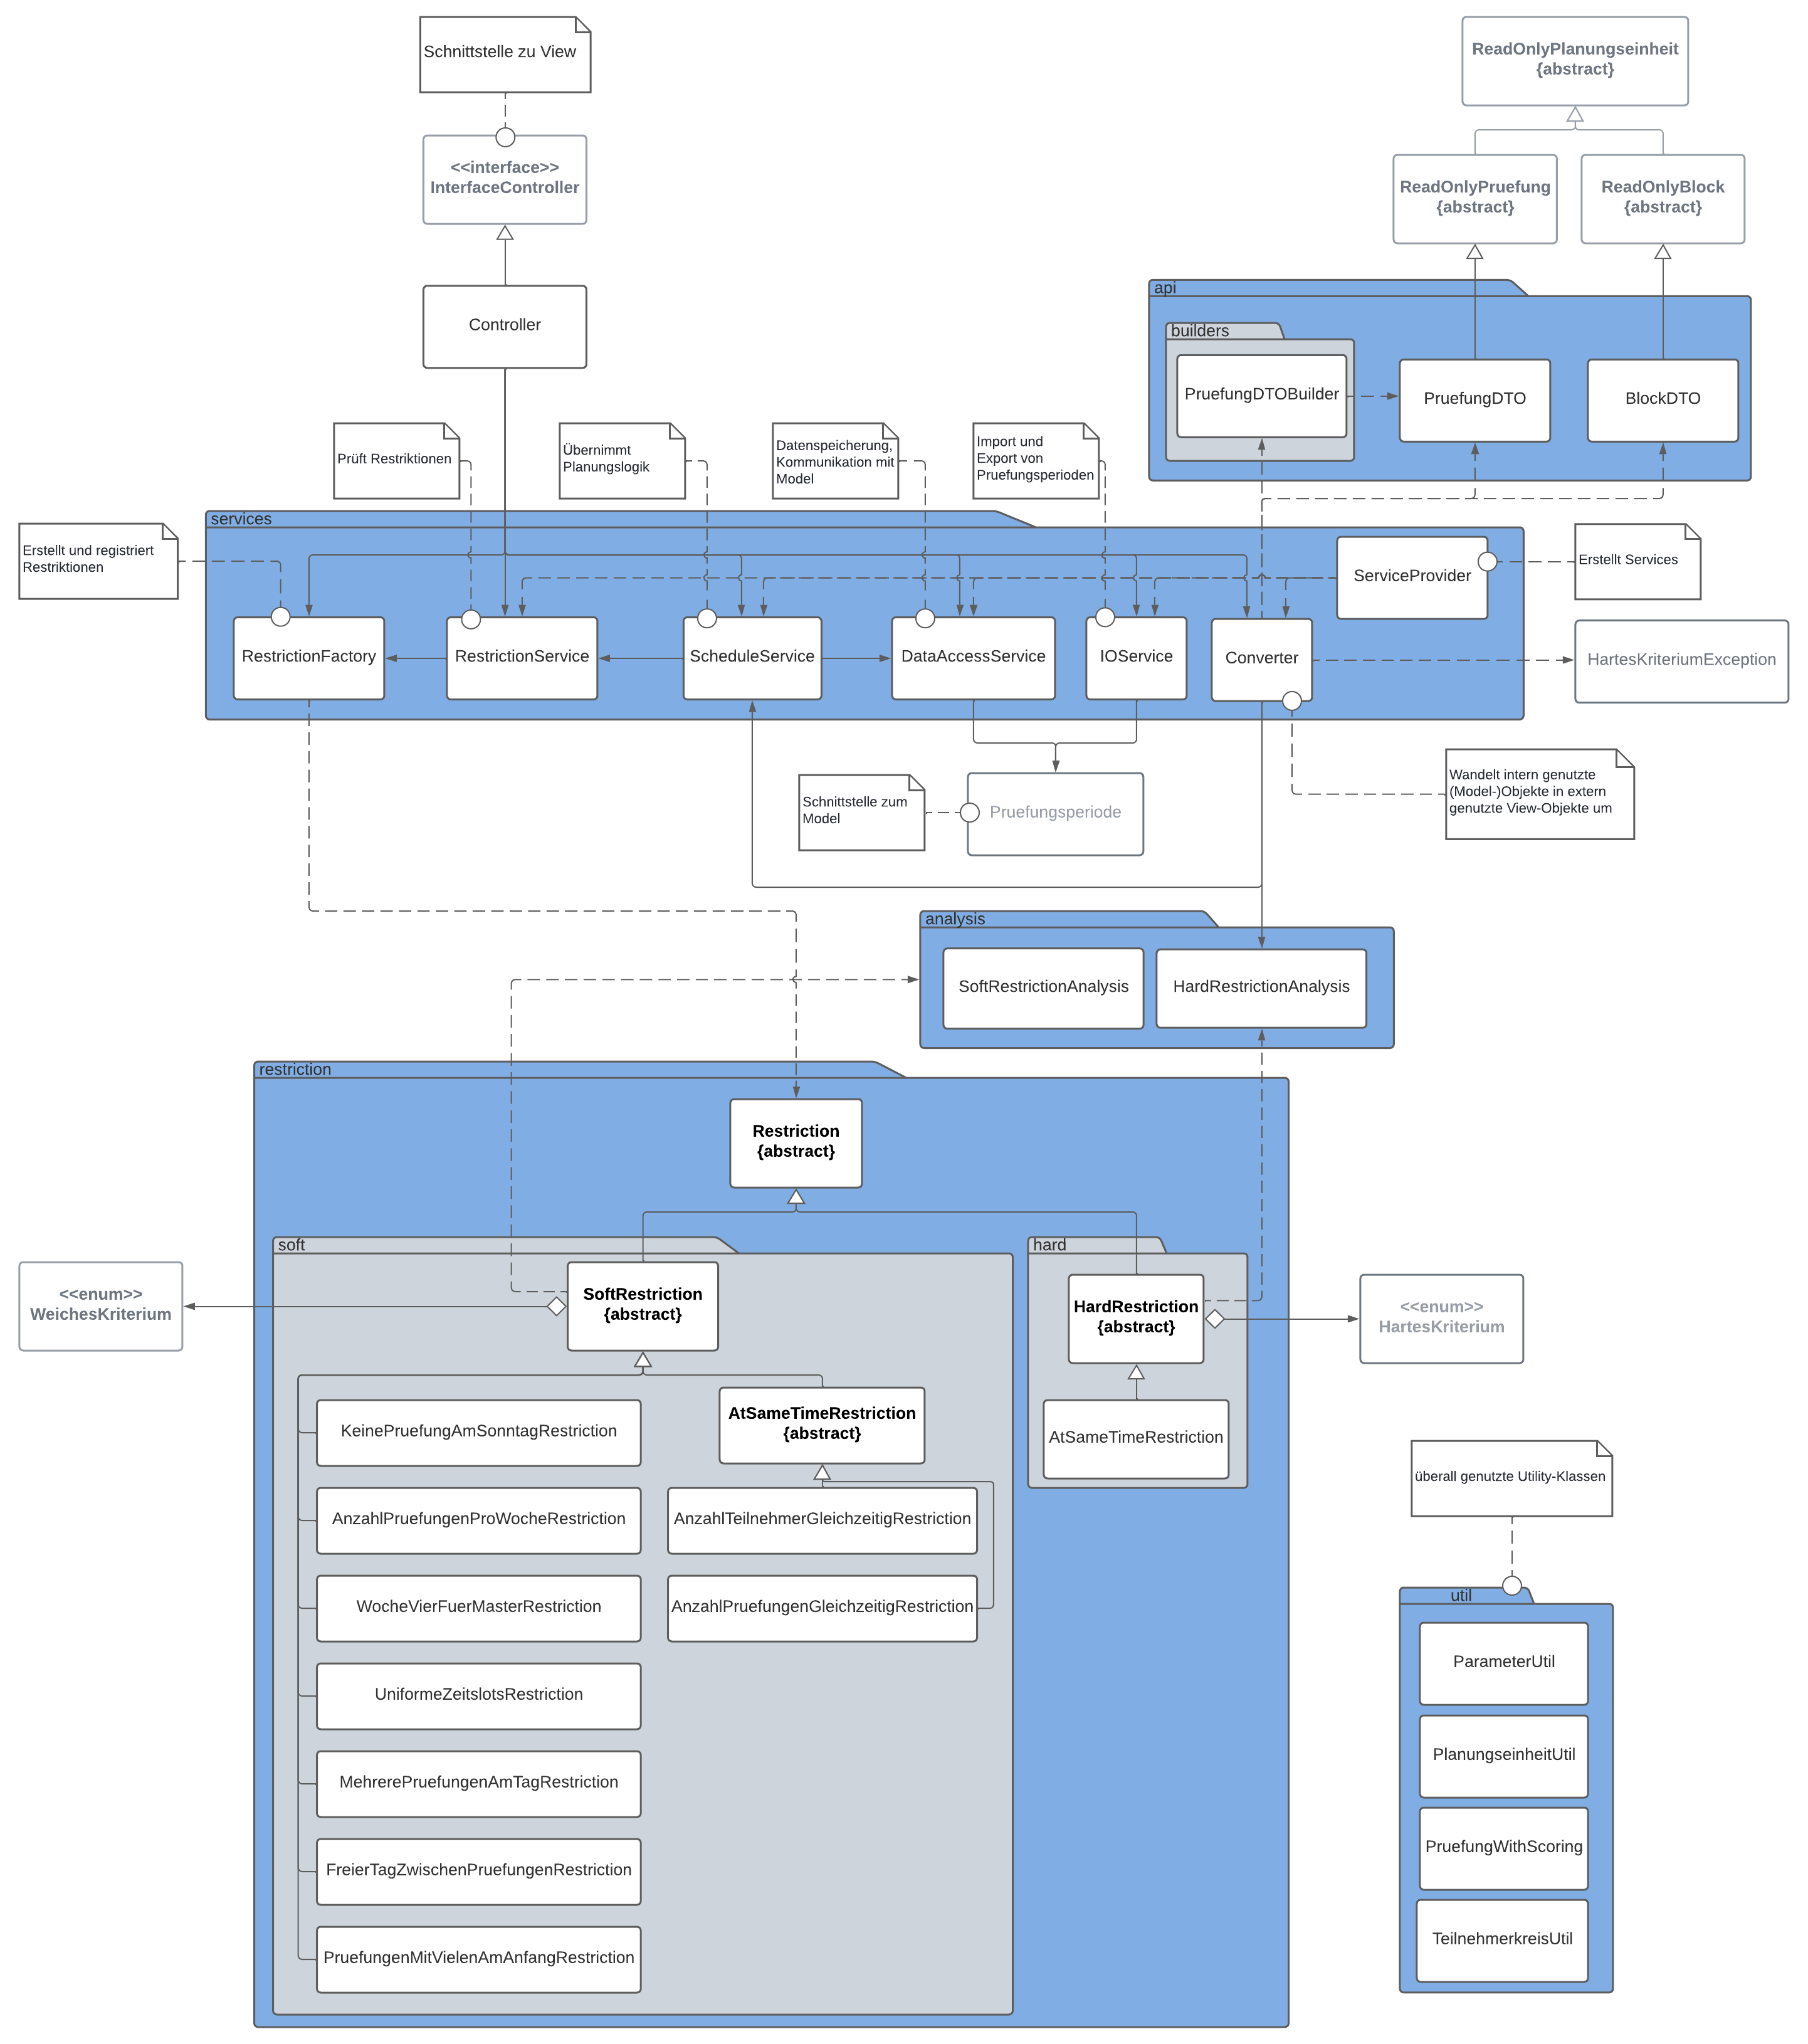
\includegraphics[width=1.25\textwidth]{extra/controller_2_uml}}%
    \end{center}

\clearpage
Den Einstieg des Projekts von View-Seite bildet die Klasse \enquote{Controller}.
Das Projekt selbst gliedert sich in fünf Haupt-Pakete, wobei sich die Hauptfunktionalität
auf die Pakete \enquote{services} und \enquote{restriction} beschränkt.

Die einzelnen Services dienen der logischen Trennung der im Controller angebotenen Funktionalität.


